\documentclass[a4paper]{article}

\usepackage{amsmath}
\usepackage{amssymb}
\usepackage{graphicx}
\usepackage{tikz}
\usetikzlibrary{arrows}
\usepackage{verbatim}
%\usepackage{sfmath}
\usepackage{psfrag}
\usepackage{here} 
\usepackage{subfigure} 

\usepackage{hyperref}
\usepackage{xcolor}
\usepackage{tcolorbox}

\title{Práctica 3}
\author{Javier Izquierdo Hernández}
\date{\today}

%\renewcommand\sfdefault{phv}     %use helvetica for sans serif
\renewcommand{\familydefault}{\sfdefault}
\renewcommand{\familydefault}{cmss}

\topmargin = 0pt
\textheight = 620pt
\textwidth = 370pt


\begin{document}
	\begin{titlepage}
		\centering
		{
\includegraphics[width=0.3\textwidth]{figures/logo}\par}
		\vspace{1cm}
		{\bfseries\LARGE Universidad Rey Juan Carlos \par}
		\vspace{1cm}
		{\scshape\Large E.T.S. Ingeniería de Telecomunicación \par}
		\vspace{3cm}
		{\scshape\Huge Ingeniería de Control \par}
		\vspace{3cm}
		{\itshape\Large Práctica 3 \par}
		\vfill
		{\Large Autor: \par}
		{\Large Javier Izquierdo Hernández \par}
		\vfill
		{\Large \today \par}
	\end{titlepage}

\begin{center}
\section*{\huge Pr\'actica 3}
\end{center}



Consider the robot manipulator represented in Figure~\ref{fig:PR_robot}, which moves in a vertical plane.




\begin{figure}[H]
\begin{center}
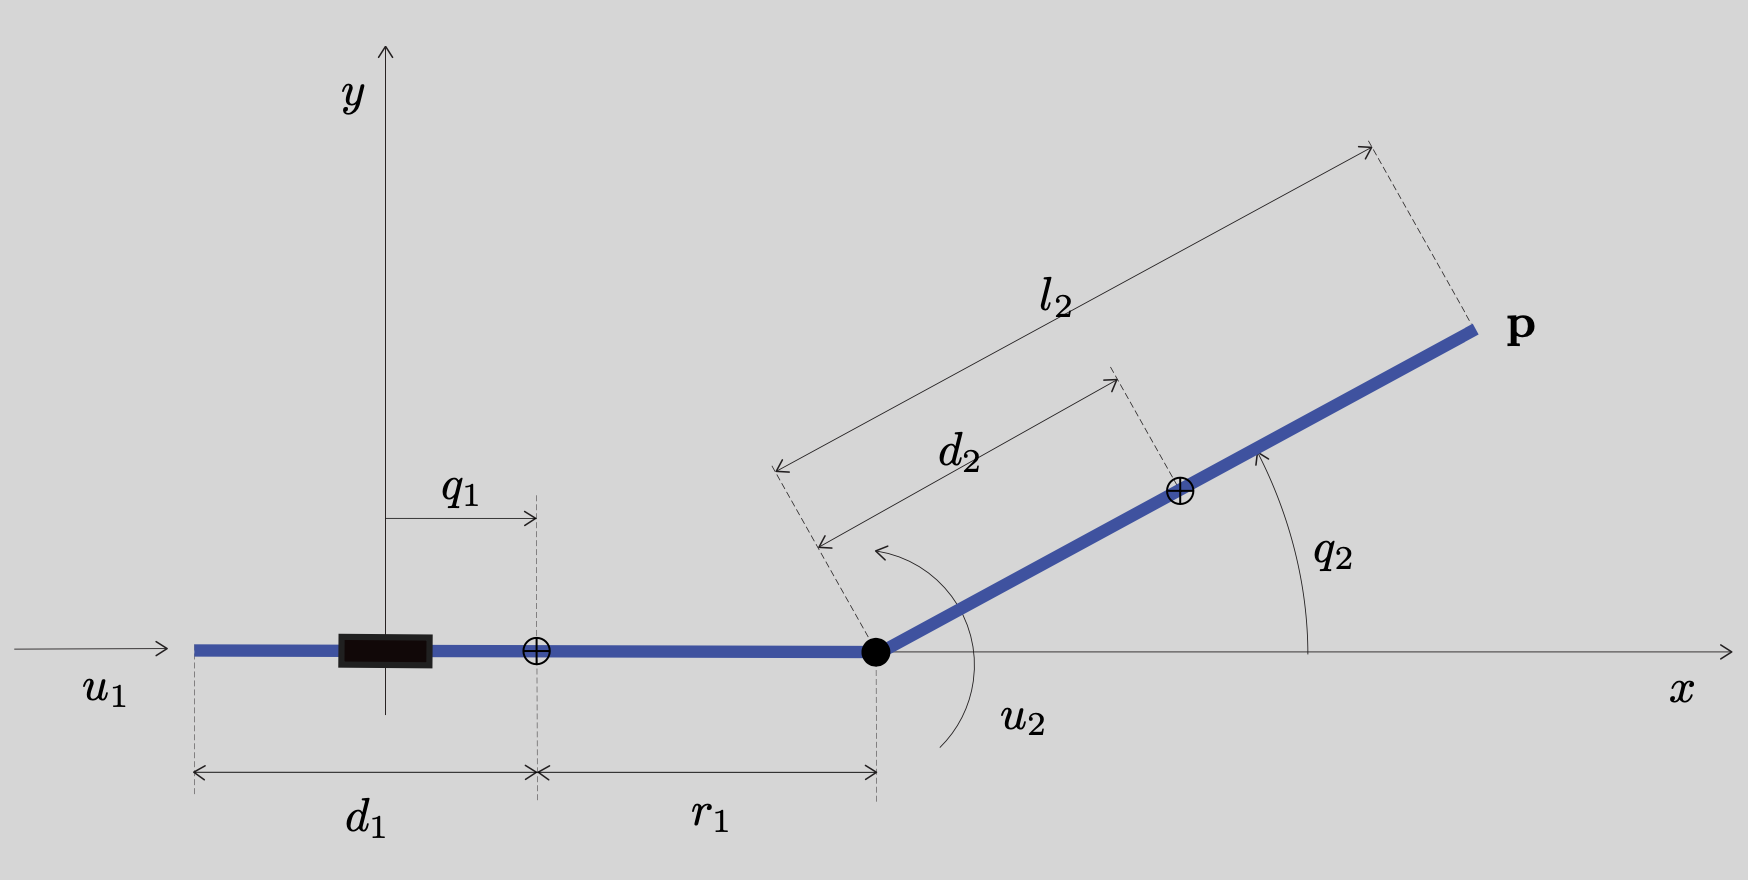
\includegraphics[width=0.99\textwidth]{figures/figure_1}
\caption{Planar vertical robot manipulator.}
\label{fig:PR_robot}
\end{center}
\end{figure} 


\noindent
The dynamic model of this robotic system is represented by the
second order differential equation 
\begin{equation*}
\mathbf{B}(\mathbf{q}) \ddot{\mathbf{q}}+ \mathbf{C}(\mathbf{q}, \dot{\mathbf{q}}) + \mathbf{N}(\mathbf{q}) = \mathbf{u},
\end{equation*}
where the matrices $\mathbf{B}(\mathbf{q})$, $\mathbf{C}(\mathbf{q}, \dot{\mathbf{q}})$, and $\mathbf{N}(\mathbf{q})$ have the following expressions
\begin{eqnarray*}
\mathbf{B}(\mathbf{q}) &=&
\begin{bmatrix}
m_1 + m_2 &-m_2 d_2 \sin ( q_2)\\
-m_2 d_2 \sin (q_2) & I_2 + m_2 d_2^2
\end{bmatrix},\\
\mathbf{C}(\mathbf{q}, \dot{\mathbf{q}}) 
&=& 
\begin{bmatrix} 
-m_2 d_2 \cos(q_2) \dot{q}_2^2\\
0
\end{bmatrix},\\
\mathbf{N}(\mathbf{q}) 
&=& 
\begin{bmatrix}
0\\
m_2 g d_2 \cos(q_2) 
\end{bmatrix}.
\end{eqnarray*}
The vector 
$
\mathbf{q} =
(
q_1, q_2
)^T
$ 
is the vector of configuration variables, where 
$q_1$ is the linear position of the center of mass of link 1 with respect to the $y$ axis of the reference frame $\{x, y\}$ and 
$q_2$ is the angular position of link 2 with respect to link 1 as illustrated in Figure~\ref{fig:PR_robot}. 
The
vector
$
\dot{\mathbf{q}} =
(\dot{q}_1,
\dot{q}_2)^T
$ 
is the vector of joint velocities, where 
$\dot{q}_1$ is the linear velocity of link 1 and
$\dot{q}_2$ is the angular velocity of link 2.
The vector
$
\ddot{\mathbf{q}} =
(\ddot{q}_1,
\ddot{q}_2)^T
$
is the vector of joint velocities, where 
$\ddot{q}_1$ is the linear acceleration of link 1 and
$\ddot{q}_2$ is the angular acceleration of link 2,
The control inputs of the system are
$
\mathbf{u} =
(u_1,
u_2)^T
$,
where $u_1$ is the force applied by the actuator at joint  $1$, and
$u_2$ is the torque applied by the actuator at joint  $2$. 
$l_1$ is the length of link 1,
$l_2$ is the length of link 2,
$m_1$ is the mass of link 1,  
$m_2$ is the mass of link 2,
$I_1$ is the barycentric moment of inertia of link 1, and
$I_2$ is the barycentric moment of inertia of link 2.
Distances $d_1$, $r_1$, and $d_2$ are defined in Figure~\ref{fig:PR_robot}.
The parameters of the dynamic model of the robot manipulator are 
$l_1 = 1$ [m],
$l_2 = 1$ [m],
$m_1 = 1$ [kg],
$m_2 = 1$ [kg],
$I_1 = 1$  [kg $\text{m}^2$],
$I_2 = 1$ [kg $\text{m}^2$],
$d_1 = \frac{l_1}{2}$ [m],
$r_1 = \frac{l_1}{2}$ [m],
$d_2 = \frac{l_2}{2}$ [m].
Consider the following two robotic tasks.

\begin{itemize}


\item[a)] Pick and place task: move iteratively the end effector $\mathbf{p}$ between the setpoints 
$\mathbf{p}_A = (1, 0.75)^T$ [m] and 
$\mathbf{p}_B = (1.5, -0.75)^T$ [m]. The motions must be rest to rest.


\item[b)]
Tracking task: follow with the end effector a setpoint $\mathbf{w}$ describing the target line segment from $\mathbf{p}_A = (1, 0.75)^T$ [m] to
$\mathbf{p}_B = (1.5, -0.75)^T$ [m], which moves with constant linear velocity $0.1$ [m/s]. 



\end{itemize}

\noindent
Suppose that, in both cases, at $t=0$ [s] the position of the end effector is 
$
\mathbf{p} = \mathbf{p}_A
$.





\begin{itemize}

\item[1)] Compute the kinetic and potential energy of the two links of the robot manipulator. (Contesta en el informe)

\item[2)] 
Compute the state space representation of the dynamics of the robot manipulator in which $\mathbf{x} = (x_1,x_2,x_3,x_4)^T= (q_1, q_2, \dot{q}_1, \dot{q}_2)^T$, where distances are measured in [m], angles in [rad], linear velocities in [m/s], and angular velocities in [rad/s]. (Contesta en el informe y sube el c\'odigo Matlab a Aula Virtual en el fichero answer\_2.m)

\item[3)]
Compute the relation between the configuration variables 
$\mathbf{q}$ and the position of the end effector $\mathbf{p} = (p_1, p_2)^T$. (Contesta en el informe y sube el c\'odigo Matlab a Aula Virtual en el fichero answer\_3.m)

\item[4)]
Compute the relation between the position of the end effector $\mathbf{p}$ and 
the configuration variables  $\mathbf{q}$. Compute the values of the configuration variables 
that correspond to $\mathbf{p} =\mathbf{p} _A$ and $\mathbf{p} =\mathbf{p}_B$. (Contesta en el informe y sube el c\'odigo Matlab a Aula Virtual en el fichero answer\_4.m)

\item[5)]
Compute the relation between the joint velocities $\dot{\mathbf{q}}$ 
and the velocity of the end effector $\dot{\mathbf{p}}$. (Contesta en el informe y sube el c\'odigo Matlab a Aula Virtual en el fichero answer\_5.m)

\item[6)]
Compute the relation between the velocity of the end effector $\dot{\mathbf{p}}$ and the joint velocities $\dot{\mathbf{q}}$. 
Suppose that the robot manipulator is ready to execute the tracking task, that is, the position of the end effector is $\mathbf{p} =\mathbf{p} _A$. Compute the initial joint velocities to execute this task. (Contesta en el informe y sube el c\'odigo Matlab a Aula Virtual en el fichero answer\_6.m)

\item[7)] 
Compute the time derivative of the Jacobian matrix. (Contesta en el informe y sube el c\'odigo Matlab a Aula Virtual en el fichero answer\_7.m)


\item[8)] Design a controller based on the feedback linearization method to execute the pick and place task. Write a \texttt{Matlab} code that implements the controller to execute the task. Show, plotting the relevant variables and an animation, that the controller satisfies the specifications. (Contesta en el informe y sube el c\'odigo \texttt{Matlab} a Aula Virtual en la carpeta answer\_8)


\item[9)] Design a controller based on the feedback linearization method to execute the tracking task. Compute the duration of the manoeuvre. Write a \texttt{Matlab} code that implements the controller to execute the task. Show, plotting the relevant variables and an animation, that the controller satisfies the specifications.  (Contesta en el informe y sube el c\'odigo \texttt{Matlab} a Aula Virtual en la carpeta answer\_9)



\end{itemize}

\bigskip

\textcolor{red}{Justifica todas las respuestas}


\newpage

\section*{Solution}

\begin{itemize}

\item[1)] {\color{gray} Compute the kinetic and potential energy of the two links of the robot manipulator. (Contesta en el informe)}


\bigskip

Primero calculamos la energía cinética $T$:
\begin{itemize}
	\item Brazo 1, solo tiene lineal porque solo se mueve sobre el eje x: 
	\begin{center}
		$T_{B_{1}} = \frac{1}{2}m_{1}\dot{q_{1}}^2$
	\end{center}
	\item Brazo 2, componente de rotación porque el brazo 2 rota:
	\begin{center}
		$T_{B_{2_{Rot}}} = \frac{1}{2}I_{2}\dot{q_{2}}^2$
	\end{center}
	\item Brazo 2, componente lineal en x porque se mueve sobre el eje x: 
	\begin{center}
		$T_{B_{2_{x}}} = \frac{1}{2}m_{2}(\frac{d}{dt}(q_{1}+r_{1}+l_{2}\ cos(q_{2})))^2$	
	\end{center}
	\item Brazo 2, componente lineal en y porque se desplaza en el eje y: 
	\begin{center}
		$T_{B_{2_{y}}} = \frac{1}{2}m_{2}(\frac{d}{dt}(l_{2}\ sin(q_{2})))^2$
	\end{center}
	\item Brazo 2:
	\begin{center} 
		$T_{B_{2}} = T_{B_{2_{Rot}}} + T_{B_{2_{x}}} + T_{B_{2_{y}}}$
	\end{center}
\end{itemize}
Como se puede apreciar, la componente lineal de la esfera ha sido dividida en 2 ya que se mueve sobre los 2 ejes, no solo en uno.\\
\begin{center}
	$T = T_{B_{1}} + T_{B_{2}} =$\\
	
	$\frac{1}{2}m_{1}\dot{q_{1}}^2 + \frac{1}{2}I_{2}\dot{q_{2}}^2 + \frac{1}{2}m_{2}(\frac{d}{dt}(q_{1}+r_{1}+l_{2}\ cos(q_{2})))^2 + \frac{1}{2}m_{2}(\frac{d}{dt}(l_{2}\ sin(q_{2})))^2 =$\\
	 
	$\frac{1}{2}m_{1}\dot{q_{1}}^2 + \frac{1}{2}I_{2}\dot{q_{2}}^2 + \frac{1}{2}m_{2}(\dot{q_{1}}\ - l_{2}\ \dot{q_{2}}\ sin(q_{2}))^2 + \frac{1}{2}m_{2}(l_{2}\ \dot{q_{2}}\ cos(q_{2}))^2 =$
	
	$m_{1}\dot{q_{1}}^2 + \frac{1}{2}I_{2}\dot{q_{2}}^2 + m_{2}\ l_{2}^2\ \dot{q_{2}}^2 - m_{2}\ l_{2}\ \dot{q_{1}}\ \dot{q_{2}}
	$
\end{center}

Por último obtenemos la energía potencial del sistema $V$. Solo brazo 2 tiene energía potencial:
\begin{center}
	$V = m_{2}\ g\ l_{2}\ sin(q_{2})$
\end{center}

\bigskip


\item[2)] 
 {\color{gray} Compute the state space representation of the dynamics of the robot manipulator in which $\mathbf{x} = (x_1,x_2,x_3,x_4)^T= (q_1, q_2, \dot{q}_1, \dot{q}_2)^T$, where distances are measured in [m], angles in [rad], linear velocities in [m/s], and angular velocities in [rad/s]. (Contesta en el informe y sube el c\'odigo Matlab a Aula Virtual en el fichero answer\_2.m)}
 
 \bigskip

Para poder calcular la representación en el espacio de estados, necesitamos conocer $\ddot{q}$, para así poder conseguir $\dot{x}$. Luego, para obtener $\ddot{q}$ despejamos de:

\begin{center}
	$B(q)\ddot{q} + C(q,\dot{q}) + N(q) = u$\\
	$B^{-1}(q)B(q)\ddot{q} + B^{-1}(q)C(q,\dot{q}) + B^{-1}(q)N(q) = B^{-1}(q)u$
	$\ddot{q} + B^{-1}(q)C(q,\dot{q}) + B^{-1}(q)N(q) = B^{-1}(q)u$
	$\ddot{q} = B^{-1}(q)u - B^{-1}(q)C(q,\dot{q}) - B^{-1}(q)N(q)$
\end{center}

Además como sabemos que $\dot{q_{1}} = x_{3}$ y que $\dot{q_{2}} = x_{4}$ el espacio de estados quedaría así:

\begin{center}
	$\begin{pmatrix}
		\dot{x_{1}}\\       
		\dot{x_{2}}\\       
	\end{pmatrix} = \begin{pmatrix}
		\dot{q_{1}}\\       
		\dot{q_{2}}\\      
	\end{pmatrix}$	\\
	$\begin{pmatrix}
		\dot{x_{3}}\\       
		\dot{x_{4}}\\       
	\end{pmatrix} = B^{-1}(q)u - B^{-1}(q)C(q,\dot{q}) - B^{-1}(q)N(q)$
\end{center}

\bigskip

\begin{tcolorbox}[width=12cm, title={File \texttt{answer\_2.m}}]
\begin{scriptsize}
\begin{verbatim}

syms q1 q2 dotq1 dotq2 ddotq1 ddotq2 u1 u2 x1 x2 x3 x4;
syms d1 d2 m1 m2 r1 l1 l2 I1 I2 g

B = [m1+m2, -m2*d2*sin(q2); -m2*d2*sin(q2), I2+m2*d2*d2]
invB = inv(B)

C = [-m2*d2*cos(q2)*dotq2*dotq2; 0];
N = [0;m2*g*d2*cos(q2)]

xdot= [dotq1;dotq2;-invB*C-invB*N+invB*[u1;u2]];
xdot = subs(xdot,[q1,q2,dotq1,dotq2], [x1,x2,x3,x4])

\end{verbatim}
\end{scriptsize}
\end{tcolorbox}


\item[3)]
 {\color{gray} Compute the relation between the configuration variables 
$\mathbf{q}$ and the position of the end effector $\mathbf{p} = (p_1, p_2)^T$. (Contesta en el informe y sube el c\'odigo Matlab a Aula Virtual en el fichero answer\_3.m)}

\bigskip

Para ello estudiamos la figura original, para determinar la posición del extremo para $x$ e $y$.

Para $x$ tenemos que se desplaza horizontalmente para el brazo 1 en relación con $q_{1}$ y $r_{1}$, y para el brazo 2 en relación a la longitud del brazo 2 $l_{2}$ y a su proyección en el eje x: $cos(q_{2})$.

\begin{center}
	$p_{1} = p_{x} = q_{1} + r_{1} + l_{2}cos(q_{2})$
\end{center}

Ahora, para la posición en el eje $y$, como el primer brazo no se desplaza en este eje, la posición solo estará determinada por el segundo. Luego la posición en el eje $y$ será:

\begin{center}
	$p_{2} = p_{y} = l_{2}sin(q_{2})$
\end{center}

Con todo esto tenemos que el extremo se encuentra en la posición:

\begin{center}
	$p = \begin{pmatrix}
		p_{1}\\       
		p_{2}\\       
	\end{pmatrix} = \begin{pmatrix}
		p_{x}\\       
		p_{y}\\       
	\end{pmatrix} = \begin{pmatrix}
		q_{1} + r_{1} + l_{2}cos(q_{2})\\       
		l_{2}sin(q_{2})\\       
	\end{pmatrix}$
\end{center}

\bigskip

\begin{tcolorbox}[width=12cm, title={File \texttt{answer\_3.m}}]
\begin{scriptsize}
\begin{verbatim}

p1 = q1 + r1 + l2*cos(q2);
p2 = l2*sin(q2);

\end{verbatim}
\end{scriptsize}
\end{tcolorbox}


\item[4)]
 {\color{gray} Compute the relation between the position of the end effector $\mathbf{p}$ and 
the configuration variables  $\mathbf{q}$. Compute the values of the configuration variables 
that correspond to $\mathbf{p} =\mathbf{p} _A$ and $\mathbf{p} =\mathbf{p}_B$. (Contesta en el informe y sube el c\'odigo Matlab a Aula Virtual en el fichero answer\_4.m)}

\bigskip

Usamos Matlab para resolver las ecuaciones obtenidas en el apartado anterior, para así obtener los valores iniciales de $q_{1} = x_{1}$ y de $q_{2} = x_{2}$.

Primero resolvemos para $ p = \begin{pmatrix}
	1\\       
	0.75\\       
\end{pmatrix}$ y obtenemos 2 valores posibles para $q_{1} = \begin{pmatrix}
1.16\\       
-0.16\\       
\end{pmatrix}$ y $q_{2}=\begin{pmatrix}
2.29\\       
0.85\\       
\end{pmatrix}$, pero de estos solo podemos elegir uno. En este caso elegimos el segundo valor de cada uno de ellos, ya que para $q_{1}$ el valor siempre debe ser menor que la longitud del brazo 1, en este caso $l_{1} = 1$, y para $q_{2}$ en este modelo sería imposible que el brazo 2 formara un ángulo de $2.29\ rad$ para llegar a ese punto, ya que para eso, el brazo 1 debería ser bastante más largo.

Luego tenemos que para llegar a $p_{A}$, $q$ tiene que valer:

\begin{center}
	$q = \begin{pmatrix}
		q_{1}\\       
		q_{2}\\       
	\end{pmatrix} = \begin{pmatrix}
		-0.16\\       
		0.85\\       
	\end{pmatrix}$
\end{center}

Por último calculamos lo mismo pero para $ p = \begin{pmatrix}
	1.5\\       
	-0.75\\       
\end{pmatrix}$ y obtenemos que $q_{1} = \begin{pmatrix}
0.34\\       
1.66\\       
\end{pmatrix}$ y $q_{2}=\begin{pmatrix}       
-0.85\\  
3.99\\     
\end{pmatrix}$. Al igual que para la $p$ anterior, en esta elegimos solo en primer valor de cada $q$. Luego queda que $q$ tiene que valer:

\begin{center}
	$q = \begin{pmatrix}
		q_{1}\\       
		q_{2}\\       
	\end{pmatrix} = \begin{pmatrix}
		0.34\\       
		-0.85\\       
	\end{pmatrix}$
\end{center}

\bigskip

\begin{tcolorbox}[width=12cm, title={File \texttt{answer\_4.m}}]
\begin{scriptsize}
\begin{verbatim}

syms q1 q2 dotq1 dotq2

d1 = 1/2;
d2 = 1/2;
m1 = 1;
m2 = 1;
r1 = 1/2;
l1 = 1;
l2 = 1;
I1 = 1;
I2 = 1;

% Para pA
p1 = q1 + r1 + l2*cos(q2) == 1;
p2 = l2*sin(q2) == 0.75;

[x1, x2] = solve([p1 p2], [q1 q2])

vpa(x1) % No puede ser mayor que 1
vpa(x2)

% Para pB
p1 = q1 + r1 + l2*cos(q2) == 1.5;
p2 = l2*sin(q2) == -0.75;

[x1, x2] = solve([p1 p2], [q1 q2])

vpa(x1) % No puede ser mayor que 1
vpa(x2)

\end{verbatim}
\end{scriptsize}
\end{tcolorbox}


\item[5)]
 {\color{gray} Compute the relation between the joint velocities $\dot{\mathbf{q}}$ 
and the velocity of the end effector $\dot{\mathbf{p}}$. (Contesta en el informe y sube el c\'odigo Matlab a Aula Virtual en el fichero answer\_5.m)}

\bigskip

Como se sabe que $\dot{p} = J(q)\dot{q}$, la relación entre $\dot{p}$ y $\dot{q}$ será la matriz jacobiana $J(q)$.

\bigskip

\begin{tcolorbox}[width=12cm, title={File \texttt{answer\_5.m}}]
\begin{scriptsize}
\begin{verbatim}

syms l1 l2 q1 q2
p1 = q1 + r1 + l2*cos(q2);
p2 = l2*sin(q2);
J = jacobian([p1, p2], [q1, q2])

\end{verbatim}
\end{scriptsize}
\end{tcolorbox}


\item[6)]
 {\color{gray} Compute the relation between the velocity of the end effector $\dot{\mathbf{p}}$ and the joint velocities $\dot{\mathbf{q}}$. 
Suppose that the robot manipulator is ready to execute the tracking task, that is, the position of the end effector is $\mathbf{p} =\mathbf{p} _A$. Compute the initial joint velocities to execute this task. (Contesta en el informe y sube el c\'odigo Matlab a Aula Virtual en el fichero answer\_6.m)}

\bigskip

Para calcular la relación inversa, simplemente despejamos $\dot{q}$ de la ecuación anterior y queda:

\begin{center}
	$J^{-1}(q)\dot{p} = J^{-1}(q)J(q)\dot{q}$\\
	$J^{-1}(q)\dot{p} = \dot{q}$
\end{center}

Luego para poder calcular la $\dot{q}$ nos queda saber cuál es $\dot{p}$. Para ello necesitamos dividir la velocidad del tracking en sus componentes $x$ e $y$, y el ángulo en el que se mueve. También es importante resaltar que como nos desplazamos hacia abajo debo de restarle $\pi$ al ángulo para así conseguir el ángulo necesario para dividirla en $x$ e $y$.

Con todo esto nos queda que:

\begin{center}
	$\dot{p} = \begin{pmatrix}
		0.0316\\       
		-0.0949\\       
	\end{pmatrix}$
\end{center}

Con $\dot{p}$ obtenida y con $J(q)$ del apartado anterior ya podemos resolver $\dot{q}$:

\begin{center}
	$\dot{q} = \begin{pmatrix}
		-0.076369\\       
		-0.14374\\       
	\end{pmatrix}$
\end{center}

\bigskip

\begin{tcolorbox}[width=12cm, title={File \texttt{answer\_6.m}}]
\begin{scriptsize}
\begin{verbatim}

syms l1 l2 q1 q2 dotq1 dotq2 r1

p1 = q1 + r1 + l2*cos(q2);
p2 = l2*sin(q2);
J = jacobian([p1, p2], [q1, q2])

% Calcular las componentes de la velocidad
ang = atan((1.5 - 1)/(-0.75 - 0.75)) - pi
max_speed = 0.1

dotpx = max_speed*sin(ang)
dotpy = max_speed*cos(ang)

J = subs(J,[q2, l2], [0.85, 1])

vpa(inv(J)*[dotpx;dotpy])

\end{verbatim}
\end{scriptsize}
\end{tcolorbox}


\item[7)] 
 {\color{gray} Compute the time derivative of the Jacobian matrix. (Contesta en el informe y sube el c\'odigo Matlab a Aula Virtual en el fichero answer\_7.m)}

\bigskip

Para calcular la derivada respecto al tiempo de la matriz jacobiana $J$, realizo un cambio de variables para tenerla con respecto a las del espacio de estado, que además las pongo con respecto al tiempo.

Luego con la función diff de Matlab calculo la derivada.

\bigskip

\begin{tcolorbox}[width=12cm, title={File \texttt{answer\_7.m}}]
\begin{scriptsize}
\begin{verbatim}

syms l2 x2(t)

J = [1, -l2*sin(x2(t)); 0,  l2*cos(x2(t))];

Jdot = diff(J,t)

\end{verbatim}
\end{scriptsize}
\end{tcolorbox}


\item[8)]  {\color{gray} Design a controller based on the feedback linearization method to execute the pick and place task. Write a \texttt{Matlab} code that implements the controller to execute the task. Show, plotting the relevant variables and an animation, that the controller satisfies the specifications. (Contesta en el informe y sube el c\'odigo \texttt{Matlab} a Aula Virtual en la carpeta answer\_8)}

\bigskip

Para esta parte he utilizado el código que habíamos usado para los últimos ejercicios y lo he modificado para que las variables fueran las de este sistema y que este se comportara de forma correcta.

El estado inicial del sistema lo he definido gracias a los resultados de los apartados anteriores (las velocidades son 0, ya que empieza en reposo):

\begin{center}
	$x = \begin{pmatrix}
		-0.16\\       
		0.85\\
		0\\
		0\\       
	\end{pmatrix}$
\end{center}

Con respecto a las matrices $K_{P}$ y $K_{D}$, las he inicializado a los siguientes valores: 

\begin{center}
	$K_{P} = \begin{pmatrix}
		10 & 0\\       
		0 & 10\\      
	\end{pmatrix}$
	$K_{D} = \begin{pmatrix}
		5 & 0\\       
		0 & 5\\      
	\end{pmatrix}$
\end{center}

Luego a la hora de ir variando entre $p_{A}$ y $p_{B}$ he usado el siguiente código para ir modificando el valor de w dependiendo de la posición del extremo y de las velocidades del sistema:

\begin{tcolorbox}[width=12cm, title={Modificar w}]
\begin{scriptsize}
\begin{verbatim}

% Es necesario el margen porque sino nunca entra
if (y(1) >= 0.99 && y(1) <= 1.01 && y(2) >= 0.74 && y(2) <= 0.76 && x(3) >= -0.01 &&
    x(3) <= 0.01 && x(4) >= -0.01 && x(4) <= 0.01)
    w = [1.5;-0.75];
elseif (y(1) >= 1.49 && y(1) <= 1.51 && y(2) >= -0.76 && y(2) <= -0.74 && x(3) >= -0.01
        && x(3) <= 0.01 && x(4) >= -0.01 && x(4) <= 0.01)
    w = [1;0.75];
end

\end{verbatim}
\end{scriptsize}
\end{tcolorbox}

En cuanto a la representación del sistema he dado al brazo 1 el color azul y al brazo 2 negro. También he puesto el extremo del brazo 1 con una cruz de color verde y al objetivo una cruz de color rojo.

\begin{center}
	\includegraphics[width=0.7\textwidth]{figures/answer\_8}
\end{center}

\bigskip


\item[9)]  {\color{gray} Design a controller based on the feedback linearization method to execute the tracking task. Compute the duration of the manoeuvre. Write a \texttt{Matlab} code that implements the controller to execute the task. Show, plotting the relevant variables and an animation, that the controller satisfies the specifications.  (Contesta en el informe y sube el c\'odigo \texttt{Matlab} a Aula Virtual en la carpeta answer\_9)}

\bigskip

Esta parte es muy similar al apartado anterior, pero cambia el estado inicial y la $w$.

Esta vez en el estado inicial si debe tener velocidad inicial, por lo tanto el sistema queda:

\begin{center}
	$x = \begin{pmatrix}
		-0.16\\       
		0.85\\
		-0.076369\\
		-0.14374\\       
	\end{pmatrix}$
\end{center}

Luego para la $w$ al aplicar la fórmula de un segmento obtengo que la $w$ es

\begin{center}
	$w = \begin{pmatrix}
		1-0.1tsin(ang)\\       
		0.75-0.1tcos(ang)\\      
	\end{pmatrix}$
\end{center}

donde el ángulo es el mismo que en apartado 6, y consecuentemente ahora $\dot{w}$ pasa de ser todo 0 a 

\begin{center}
	$\dot{w} = \begin{pmatrix}
		-0.1sin(ang)\\       
		-0.1cos(ang)\\      
	\end{pmatrix}$
\end{center}

Con este controlador conseguimos que el tiempo de la maniobra sea de 15.81 segundos.

\begin{center}
	\includegraphics[width=0.7\textwidth]{figures/answer\_9}
\end{center}

\bigskip

\end{itemize}

\end{document}